\documentclass{MyLatex}
\setlength{\headheight}{39pt}
\begin{document}

% 标题,作者
\emptitle{叶栅平台搭建中孔位加工安装说明书}
\empauthor{周雷}{}{徐弘一}
% 奇数页页眉 % 请在这里写出第一作者以及论文题目
\fancyhead[CO]{{\footnotesize 周雷: 叶栅平台空位加工说明}}


%%%%%%%%%%%%%%%%%%%%%%%%%%%%%%%%%%%%%%%%%%%%%%%%%%%%%%%%%%%%%%%%
% 关键词 摘要 首页脚注
%%%%%%%%关键词
\Keyword{M6螺纹孔, M6间隙孔,M2.5螺纹孔,M2.5间隙孔, 中等配合, 英制G1/4螺纹孔, $\Phi$1通孔}
\twocolumn[
\begin{@twocolumnfalse}
\maketitle

%%%%%%%%摘要
\begin{empAbstract}本文主要说明叶栅平台搭建中各零部件之间的配合细节。用到了M6螺纹、M2.5螺纹、英制G1/4螺纹和$\Phi$ 1测量孔。螺纹配合均采用中等配合。


\end{empAbstract}

%%%%%%%%首页角注,依次为实验时间、报告时间、学号、email
\empfirstfoot{2022-10-12}{2022-10-12}
\end{@twocolumnfalse}
]
%%%%%%%%!首页角注可能与正文重叠,请通过调整正文中第一页的\enlargethispage{-3.3cm}位置手动校准正文底部位置:
%%%%%%%%%%%%%%%%%%%%%%%%%%%%%%%%%%%%%%%%%%%%%%%%%%%%%%%%%%%%%%%%
%  正文由此开始
\wuhao 
%  分栏开始

\section{引~~言}
下文中每个标题与相对应的图纸文件名一致。加工时可以配合solidworks文件进行查阅。





\section{孔位说明}
此处列出交付的图纸名称。

主要包括“核心底DNS.SLDPRT”、“主体.SLDPRT”、“1\_1.SLDPRT”、“1\_3.SLDPRT”、“核心盖.SLDPRT”和“稳流后.SLDPRT”设计文件。
\enlargethispage{-3.3cm}



\subsection{核心底DNS.SLDPRT}

如图\ref{fig:核心底整体视图}所示,结构中包含三种孔类型。红色标记的孔为M6螺纹孔,深度没有严格定义,建议螺纹深度为10mm即可,和核心盖图纸中绿色标记的孔如图\ref{fig:核心盖}配合。绿色标记的孔为M2.5间隙孔,与翼型两侧的M2.5螺纹孔如图\ref{fig:翼型}配合。两侧的孔位均为$\Phi$1的通孔。孔详细参数如图\ref{fig:测壁通孔}所示。
\begin{figure}[H]
\centering
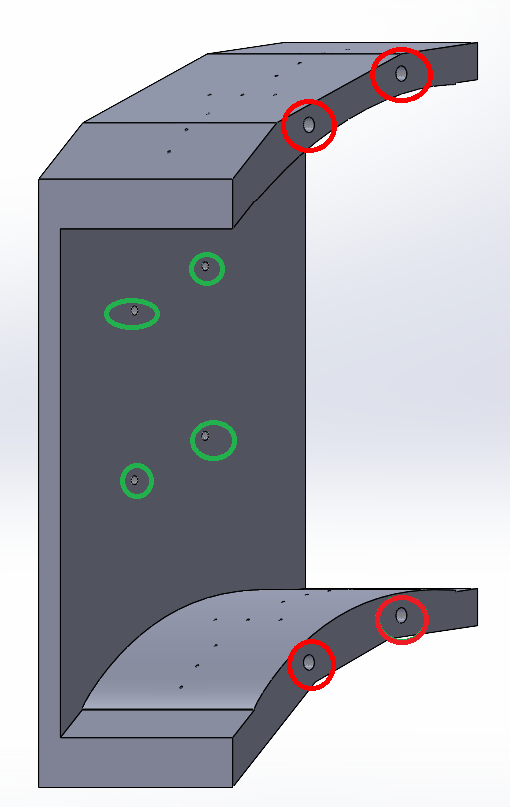
\includegraphics[width=0.8\linewidth]{./image/Zpicture/核心底整体视图.png}
\caption{核心底整体视图} \label{fig:核心底整体视图}
\end{figure}

\begin{figure}[H]
\centering
\subfigure[测壁通孔下]{
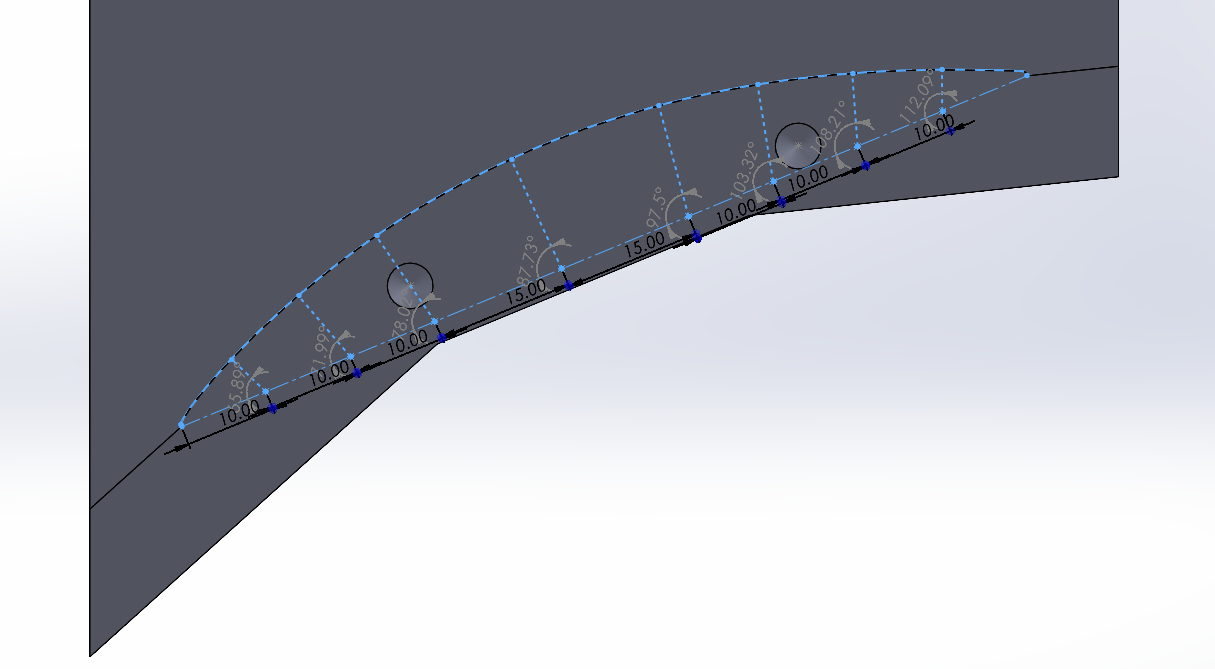
\includegraphics[width=0.8\linewidth]{./image/Zpicture/核心底侧壁1mm通孔.png}
}
\quad
\subfigure[测壁通孔上]{
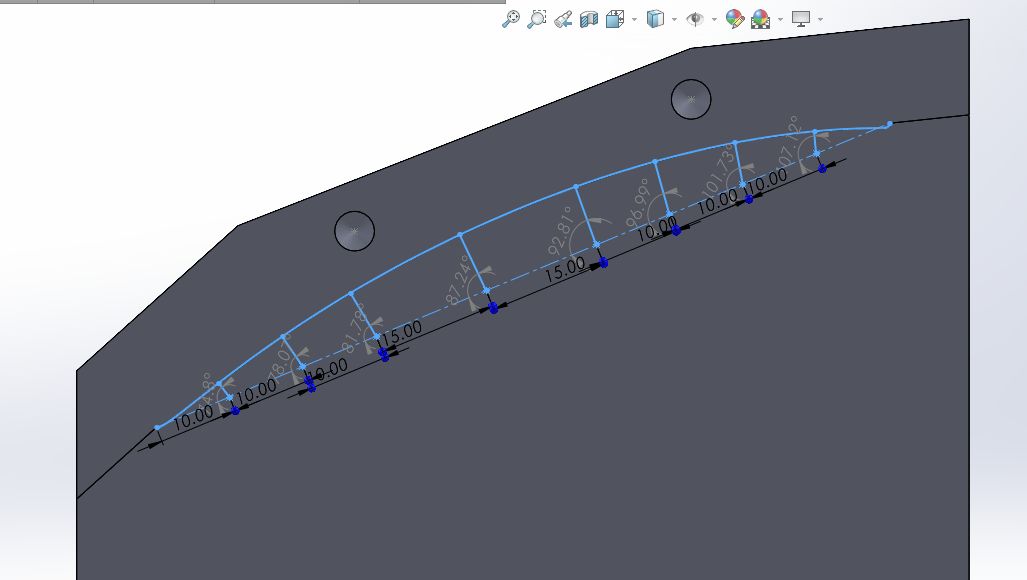
\includegraphics[width=0.8\linewidth]{./image/Zpicture/核心底侧壁1mm通孔_2.png}
}
\caption{侧面$\Phi$1mm通孔位置图} \label{fig:测壁通孔}
\end{figure}




\subsection{主体.SLDPRT}
如图\ref{fig:翼型}所示,翼型上下孔均为M2.5螺纹孔,总共4个,深度不做具体要求,按照经验加工即可。其中一侧的孔位与核心底如图\ref{fig:核心底整体视图}中M2.5间隙孔配合,另一侧与核心盖如图\ref{fig:核心盖}中的M2.5间隙孔配合。配合均采用中等配合。

\begin{figure}[H]
\centering
\subfigure[翼型]{
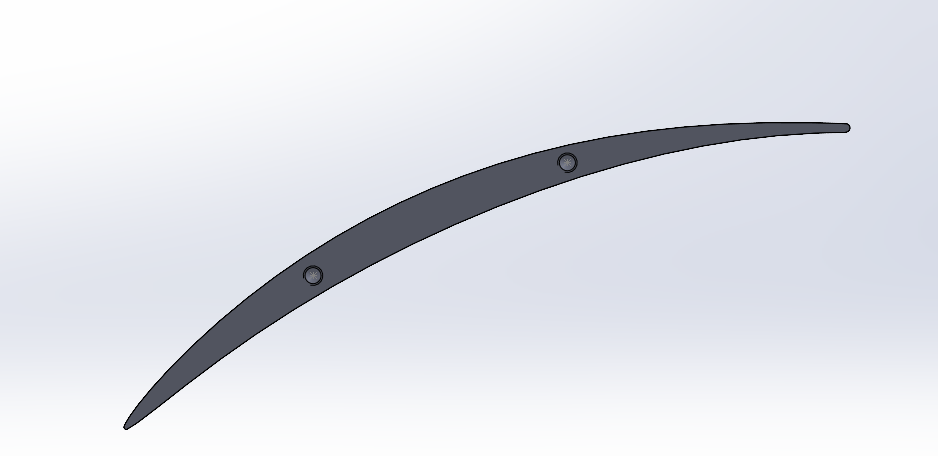
\includegraphics[width=0.8\linewidth]{./image/Zpicture/翼型.png}
}
\quad
\subfigure[翼型孔位]{
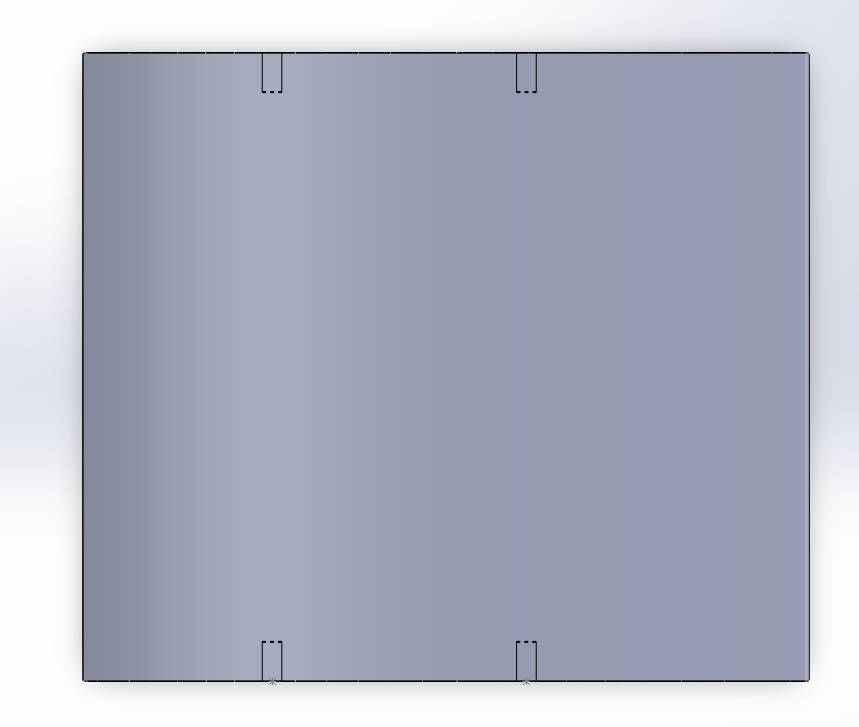
\includegraphics[width=0.8\linewidth]{./image/Zpicture/翼型孔位.png}
}
\caption{翼型孔位说明图} \label{fig:翼型}
\end{figure}

\subsection{1\_1.SLDPRT}
如图\ref{fig:上水管}所示,法兰处孔特征为M6间隙孔,中等配合,总共10个;上壁面孔特征为M6螺纹孔,总共4个,与核心盖如图\ref{fig:核心盖}中黑色标记孔配合。其中螺纹孔的深度要求为:壁面厚度为10mm,螺纹孔要求不打穿。
\begin{figure}[H]
\centering
\subfigure[上水管道整体视图]{
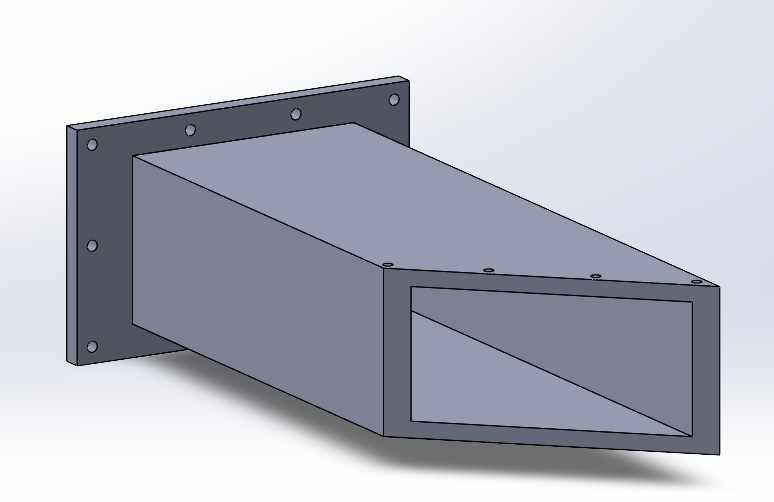
\includegraphics[width=0.8\linewidth]{./image/Zpicture/1_1整体视图.png}
}
\quad
\subfigure[上水管道孔位视图]{
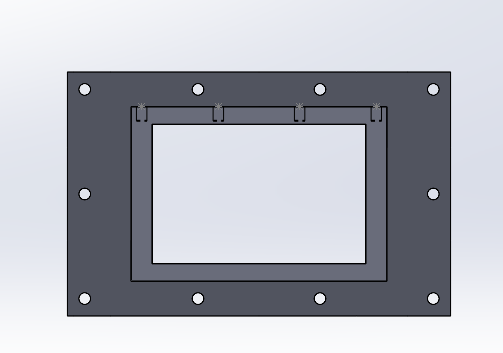
\includegraphics[width=0.8\linewidth]{./image/Zpicture/1_1孔位示意图.png}
}
\caption{上游管道} \label{fig:上水管}
\end{figure}


\subsection{1\_3.SLDPRT}
如图\ref{fig:出水管}所示,法兰处孔特征为M6间隙孔,中等配合,总共10个;上壁面孔特征为M6螺纹孔,总共4个,与核心盖如图\ref{fig:核心盖}中红色标记孔配合。其中螺纹孔的深度要求为:壁面厚度为10mm,螺纹孔要求不打穿。如图\ref{fig:底英制螺纹}所示,底部孔位为英制G1/4孔,贯穿底面。如图\ref{fig:底部槽}所示,开槽,开槽尺寸和深度参照solidworks图纸,底部孔为$\Phi$4.3的通孔,参照soldworks图纸。
\begin{figure}[H]
\centering
\subfigure[出水管道整体视图]{
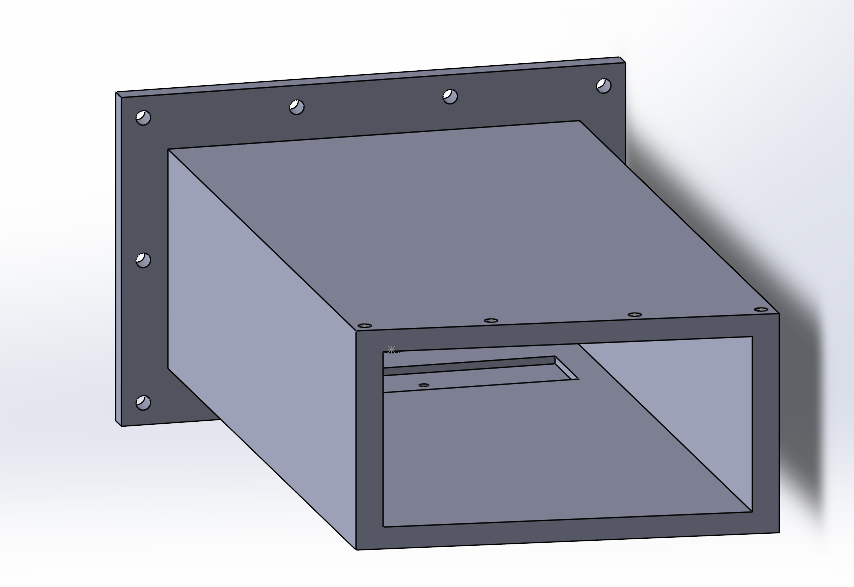
\includegraphics[width=0.8\linewidth]{./image/Zpicture/1_3整体视图.png} 
}
\quad
\subfigure[出水管道孔位视图]{
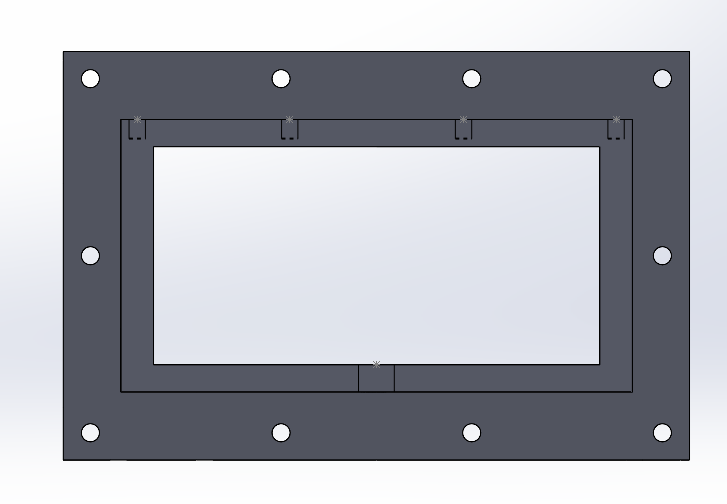
\includegraphics[width=0.8\linewidth]{./image/Zpicture/1_3孔位示意图.png}
}
\caption{下游管道} \label{fig:出水管}
\end{figure}

\begin{figure}[H]
\centering
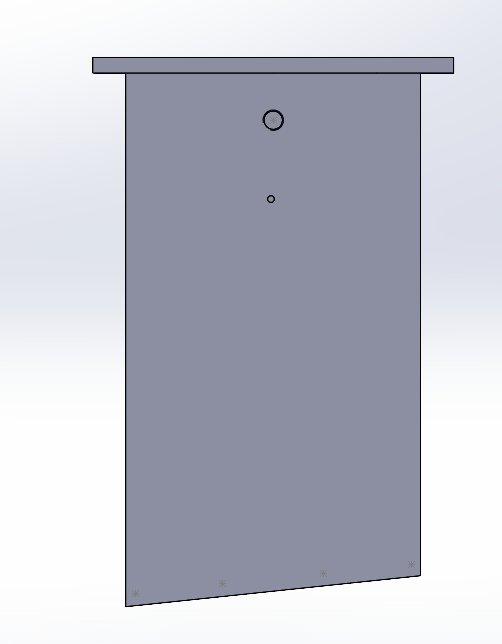
\includegraphics[width=0.8\linewidth]{./image/Zpicture/1_3底部英制螺纹孔.png}
\caption{底部英制螺纹说明} \label{fig:底英制螺纹}
\end{figure}

\begin{figure}[H]
\centering
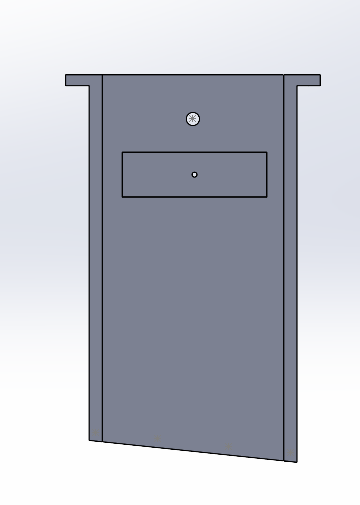
\includegraphics[width=0.8\linewidth]{./image/Zpicture/1_3底部开槽.png}
\caption{底部开槽示意图} \label{fig:底部槽}
\end{figure}

\subsection{核心盖.SLDPRT}
如图\ref{fig:核心盖}所示,孔特征均为间隙孔。黑色部分为M6间隙孔,中等配合,与图纸“1\_1.SLDPRT”中M6螺纹孔配合,如图\ref{fig:上水管}所示。

红色部分为M6间隙孔,中等配合,与图纸“1\_3.SLDPRT”中M6螺纹孔配合,如图\ref{fig:出水管}所示。

绿色部分为M6间隙孔,中等配合,与图纸“核心底.SLDPRT”中M6螺纹孔配合,如图\ref{fig:核心底整体视图}所示。

橙色部分为M2.5间隙孔,中等配合,与图纸“主体.SLDPRT”中翼型两侧的M2.5螺纹孔配合,如图\ref{fig:翼型}所示。

\begin{figure}[H]
\centering
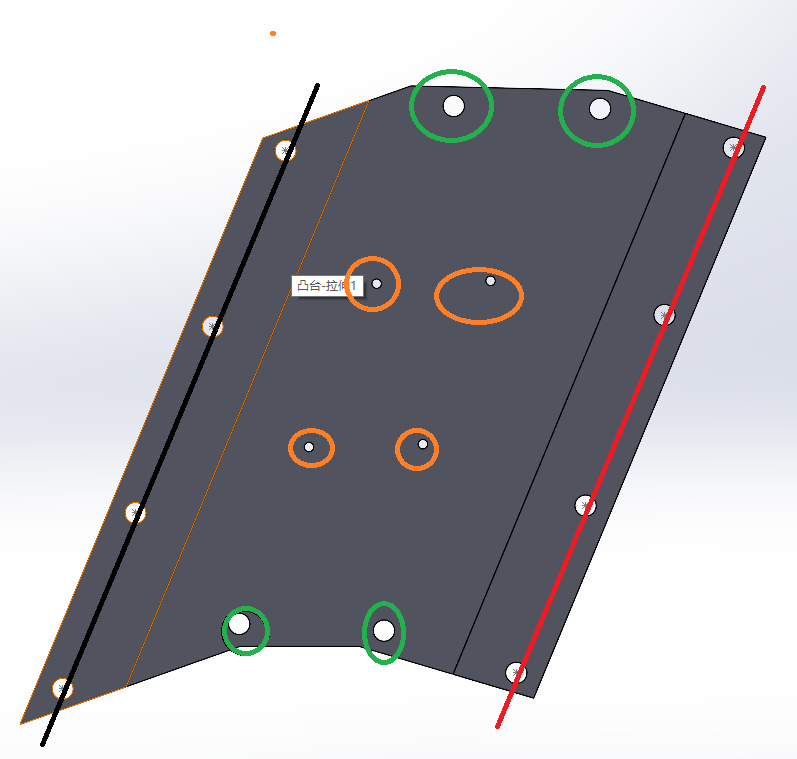
\includegraphics[width=0.8\linewidth]{./image/Zpicture/核心盖.png}
\caption{底核心盖孔位说明} \label{fig:核心盖}
\end{figure}

\subsection{稳流后.SLDPRT}
如图\ref{fig:尾部}所示,红色标记的孔特征为M6螺纹孔,孔深度可以打穿。黑色标记的孔特征为英制G1/4螺纹孔,贯穿。其余孔特征为M6间隙孔,中等配合。

\begin{figure}[H]
\centering
\subfigure[后部稳流整体视图]{
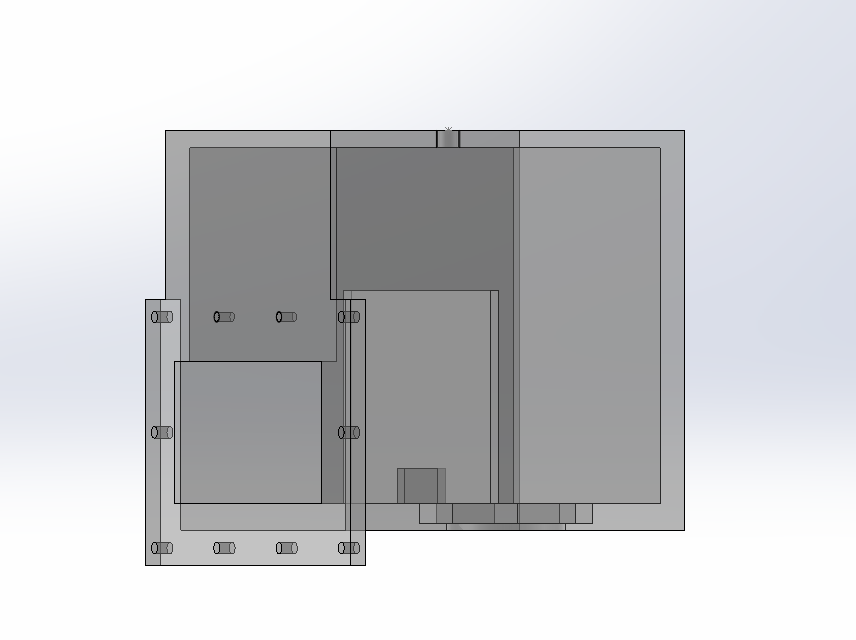
\includegraphics[width=0.8\linewidth]{./image/Zpicture/稳流后整体视图.png} 
}
\quad
\subfigure[孔位说明]{
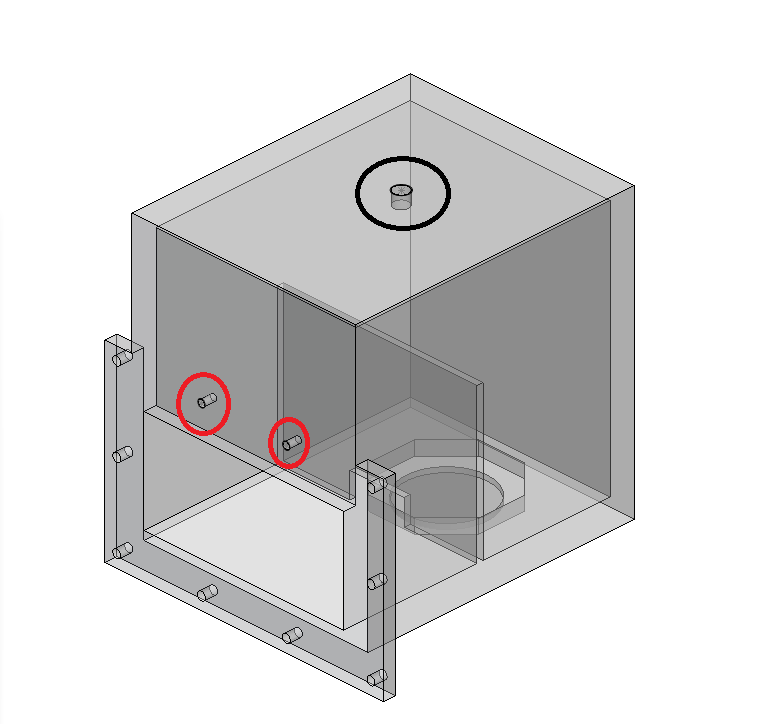
\includegraphics[width=0.8\linewidth]{./image/Zpicture/稳流后孔位说明.png}
}
\caption{尾部稳流装置} \label{fig:尾部}
\end{figure}







\section{整体视图}
整体安装图如图\ref{fig:总装}所示。
\begin{figure}[H]
\centering
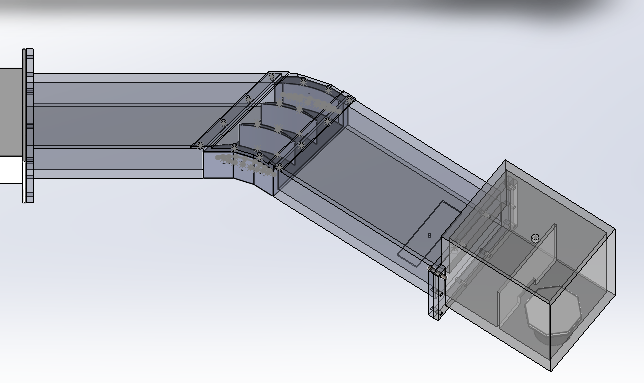
\includegraphics[width=0.8\linewidth]{./image/Zpicture/安装效果图.png}
\caption{总体安装效果图} \label{fig:总装}
\end{figure}



\section{总~~结}
有任何问题,请随时联系我。

Tel:18721290631





%\subsection{报告中表的规范}
%推荐使用标准“三线表”(如表\ref{tab:eg1}所示。),内容易混淆时可加辅助线进行辅助说明。按表格在文中出现的顺序,用阿拉伯数字对其进行编号,全文顺序编号。应%有相应的表题且每个表格前都应有相应的引出或介绍文字。

%图、表应在文中有相应表述,即图、表的号应在文中引出,以先见文后见图、表为原则。每个图、表都必须有图名、表名,并且有编号。图号、表号应全文统一连续排列,%即,应按照图1、图2……排列不应按小结编号。图片中的文字、线条应当清晰可辨,图片像素(DPI)在300以上。
%表格推荐采用全线表,表头中使用量符号/量单位形式。如表\ref{tab:eg2}所示。

\begin{table}[H]
\centering
\captionnamefont{\wuhao\bf\heiti}
\captiontitlefont{\wuhao\bf\heiti}
\caption{三线表示例} \label{tab:eg1}
\liuhao
\begin{tabular}{cccc}
\toprule
{编号} &  {直径}/\si{\metre} & {静温}/\si{\kelvin} & {时间}/min\\
\midrule 
4 & 0.0349 & 268.15 & 30\\
5 & 0.01905 & 268.15 & 30\\
\bottomrule
\end{tabular}
\end{table}

%\begin{table}[h]
%\centering
%\captionnamefont{\wuhao\bf\heiti}
%\captiontitlefont{\wuhao\bf\heiti}
%\caption{全线表示例} \label{tab:eg2}
%\liuhao
%\begin{tabular}{|c|c|c|c|c|}
%\hline
%U/V & I/mA & v/km·h$^{-1}$ & x/mm & p/MPa \\ \hline
%\textit{12} & \textit{30} & \textit{80} & \textit{55} & \textit{110} \\ \hline
%\textit{24} & \textit{34} & \textit{90} & \textit{60} & \textit{111} \\ \hline
%\end{tabular}
%\end{table}

%\subsection{报告中英文缩略语的规范}



%\subsection{外文字母}
%\subsubsection{斜体外文字母用于表示量的符号,主要用于下列场合}

%\begin{enumerate}
%\renewcommand{\labelenumi}{(\theenumi)}
%\item 变量符号、变动附标及函数。
%\item 用字母表示的数及代表点、线、面、体和图形的字母。
%\item 特征数符号,如Re (雷诺数)、Fo (傅里叶数)、Al (阿尔芬数)等。
%\item 在特定场合中视为常数的参数。
%\end{enumerate} 


%\subsubsection{正体外文字母用于表示名称及与其有关的代号,主要用于下列场合}
%\begin{enumerate}
%\renewcommand{\labelenumi}{(\theenumi)}
%\item 有定义的已知函数(例如$\sin$, $\exp$, $\ln$等)。
%\item 其值不变的数学常数(例如$\mathrm{e} = 2.718 281 8\cdots)$及已定义的算子。
%\item 法定计量单位、词头和量纲符号。
%\item 数学符号。
%\item 化学元素符号。
%\item 机具、仪器、设备和产品等的型号、代号及材料牌号。
%\item 硬度符号。
%\item 不表示量的外文缩写字。
%\item 表示序号的拉丁字母。
%\item 量符号中为区别其他量而加的具有特定含义的非量符号下角标。
%\end{enumerate} 

%\section{结~~论}



%%%%%%%%%%%%%%%%%%%%%%%%%%%%%%%%%%%%%%%%%%%%%%%%%%%%%%%%%%%%%%%%
%  参考文献
%%%%%%%%%%%%%%%%%%%%%%%%%%%%%%%%%%%%%%%%%%%%%%%%%%%%%%%%%%%%%%%%
%  参考文献按GB/T 7714-2015《文后参考文献著录规则》的要求著录. 
%  参考文献在正文中的引用方法:\cite{bib文件条目的第一行}

%\renewcommand\refname{\heiti\wuhao\centerline{参考文献}\global\def\refname{参考文献}}
%\vskip 12pt

%\let\OLDthebibliography\thebibliography
%\renewcommand\thebibliography[1]{
  %\OLDthebibliography{#1}
 % \setlength{\parskip}{0pt}
%  \setlength{\itemsep}{0pt plus 0.3ex}
%}

%{
%\renewcommand{\baselinestretch}{0.9}
%\liuhao
%\bibliographystyle{gbt7714-numerical}
%\bibliography{./TempExample}
%}



\end{document}
